\section{Tropical Rainforest}

Tropical rainforests climates or equatorial climates are characterised by frequent and heavy rainfall and are situated on or close to the equator. Because of there locality on earth there are no seasons and therefore very little temperature and illumination variance throughout the year.\\

\subsection{Resource Configuration}

Toamasina, a city in Madagascar at latitude 18\textdegree south, is the location on which climate data is based for these tests.\\

To model a loamy soil, which is common in tropical forests due to its water absorption capabilities, the soil infiltration rate is set to fifteen millimetres per hour (see figure \ref{tab:soil_types}). To model rocky cliff faces, the soil infiltration rate is set to zero when the slope angle surpasses forty degrees.\\

The configured monthly rainfall and rainfall intensity is summarized in figure \ref{fig:results_tropical_input}.

The temperature extremes configured are twenty-one degrees for June and twenty-six degrees for December, resulting in monthly temperatures outlined in figure \ref{fig:results_tropical_input}.

\begin{figure}
\center
	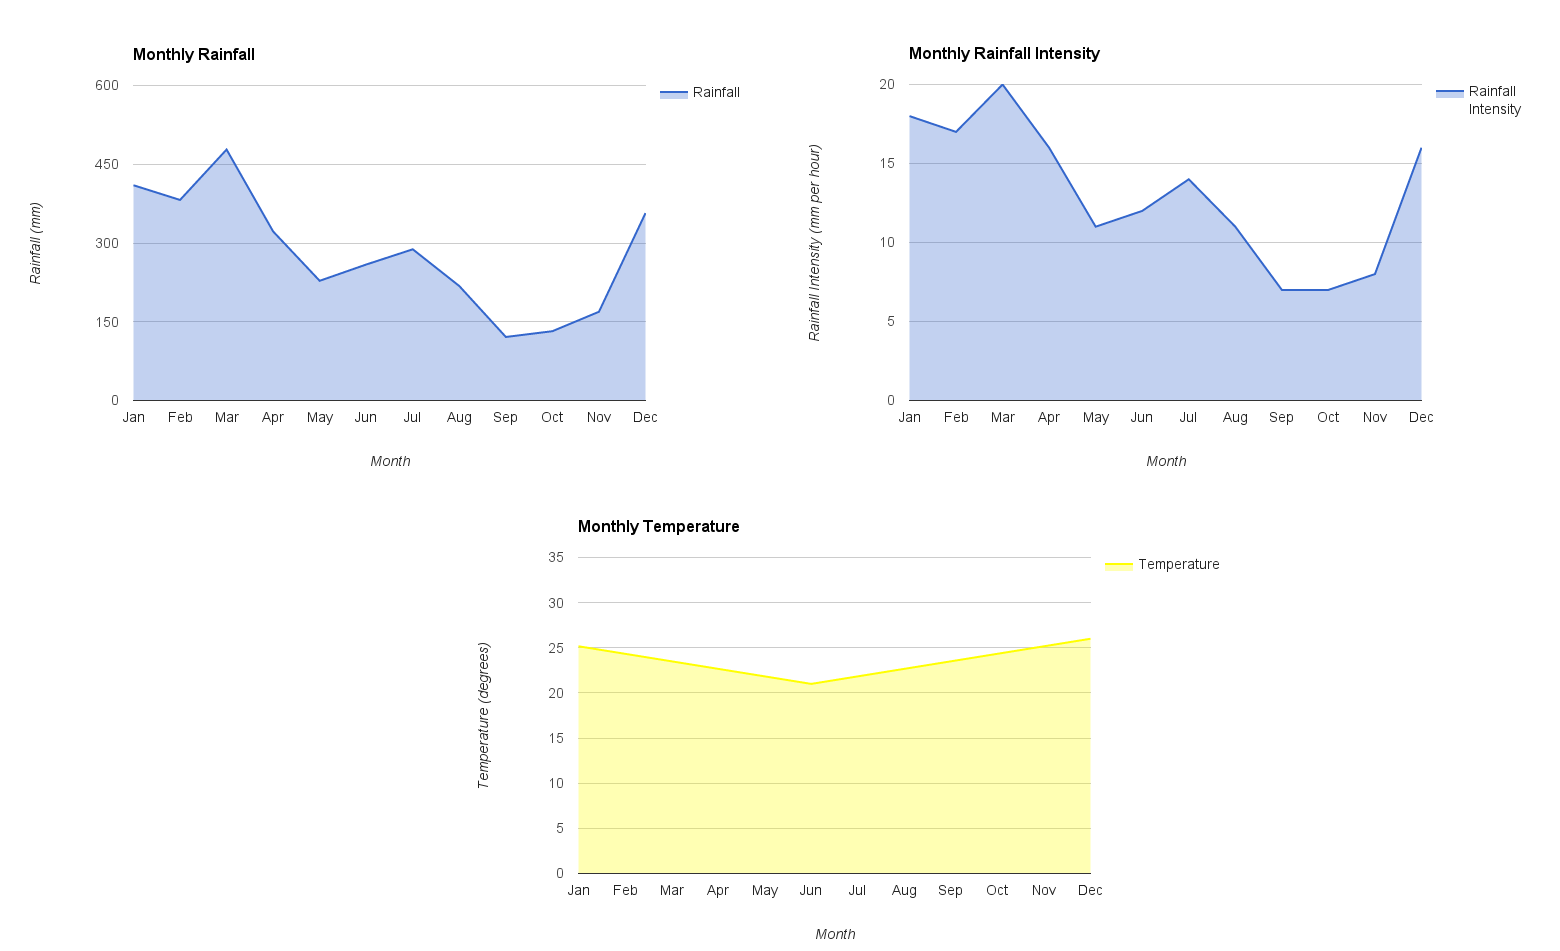
\includegraphics[width=\textwidth]{results_tropical_input.png}
	\caption{ Tropical rainforest: Input resource configurations: Rainfall (top-left), rainfall intensity (top-right) and temperature (bottom).}
	\label{fig:results_tropical_input}
\end{figure}

\subsection{Water Networks}

Given the varying monthly rainfall quantity and intensity, the resulting water networks differ for each month. Figure \ref{fig:results_tropical_water_networks} shows the water networks that form for every month of the year.

\begin{figure}
\center
	\includegraphics[width=\textwidth]{results_tropical_water_networks.png}
	\caption{ Tropical rainforest: Water networks that form on the terrain at every month. From left to right, top to bottom.}
	\label{fig:results_tropical_water_networks}
\end{figure}

\subsection{Clusters}

The number of clusters to generate is set to ten. The clustered terrain is shown in figure \ref{fig:results_tropical_terrain_clusters} and the corresponding cluster properties summarized in figure \ref{fig:results_tropical_cluster_hum_temp_illum} and table \ref{tab:results_tropical_cluster_slope_covarea}.

\begin{figure}
\center
	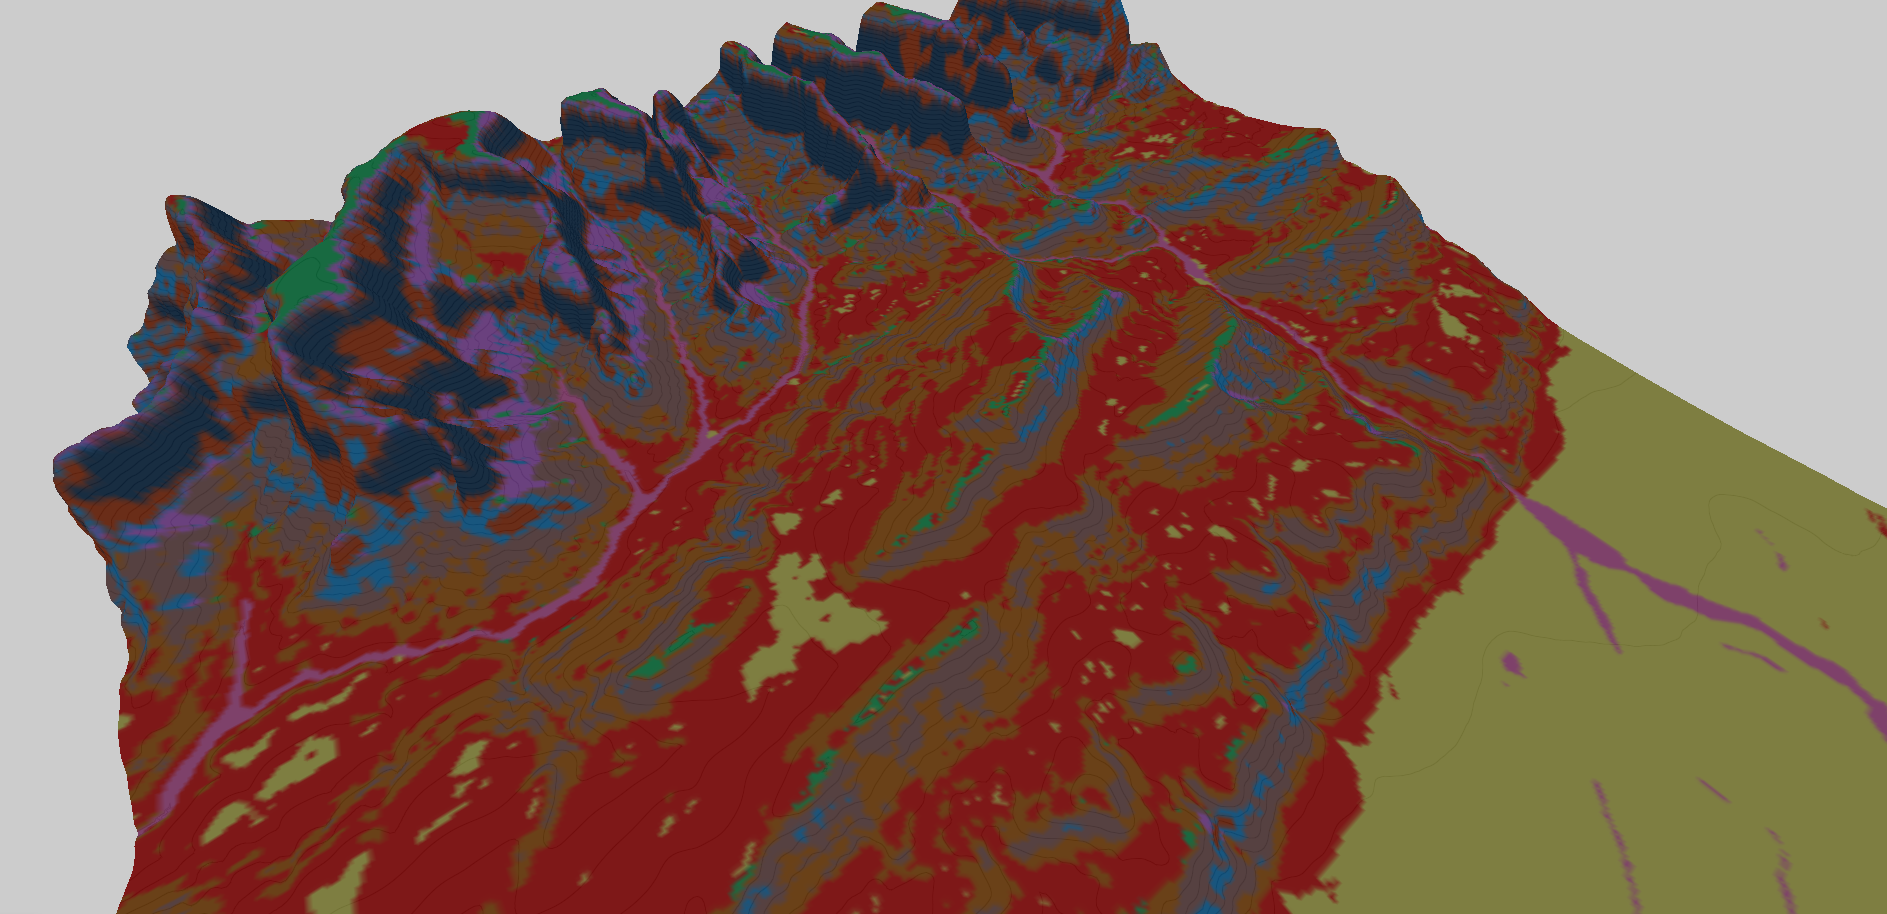
\includegraphics[width=\textwidth]{results_tropical_clusters_on_terrain.png}
	\caption{ Tropical rainforest: Resulting terrain clusters.}
	\label{fig:results_tropical_terrain_clusters}
\end{figure}

\begin{figure}
\center
	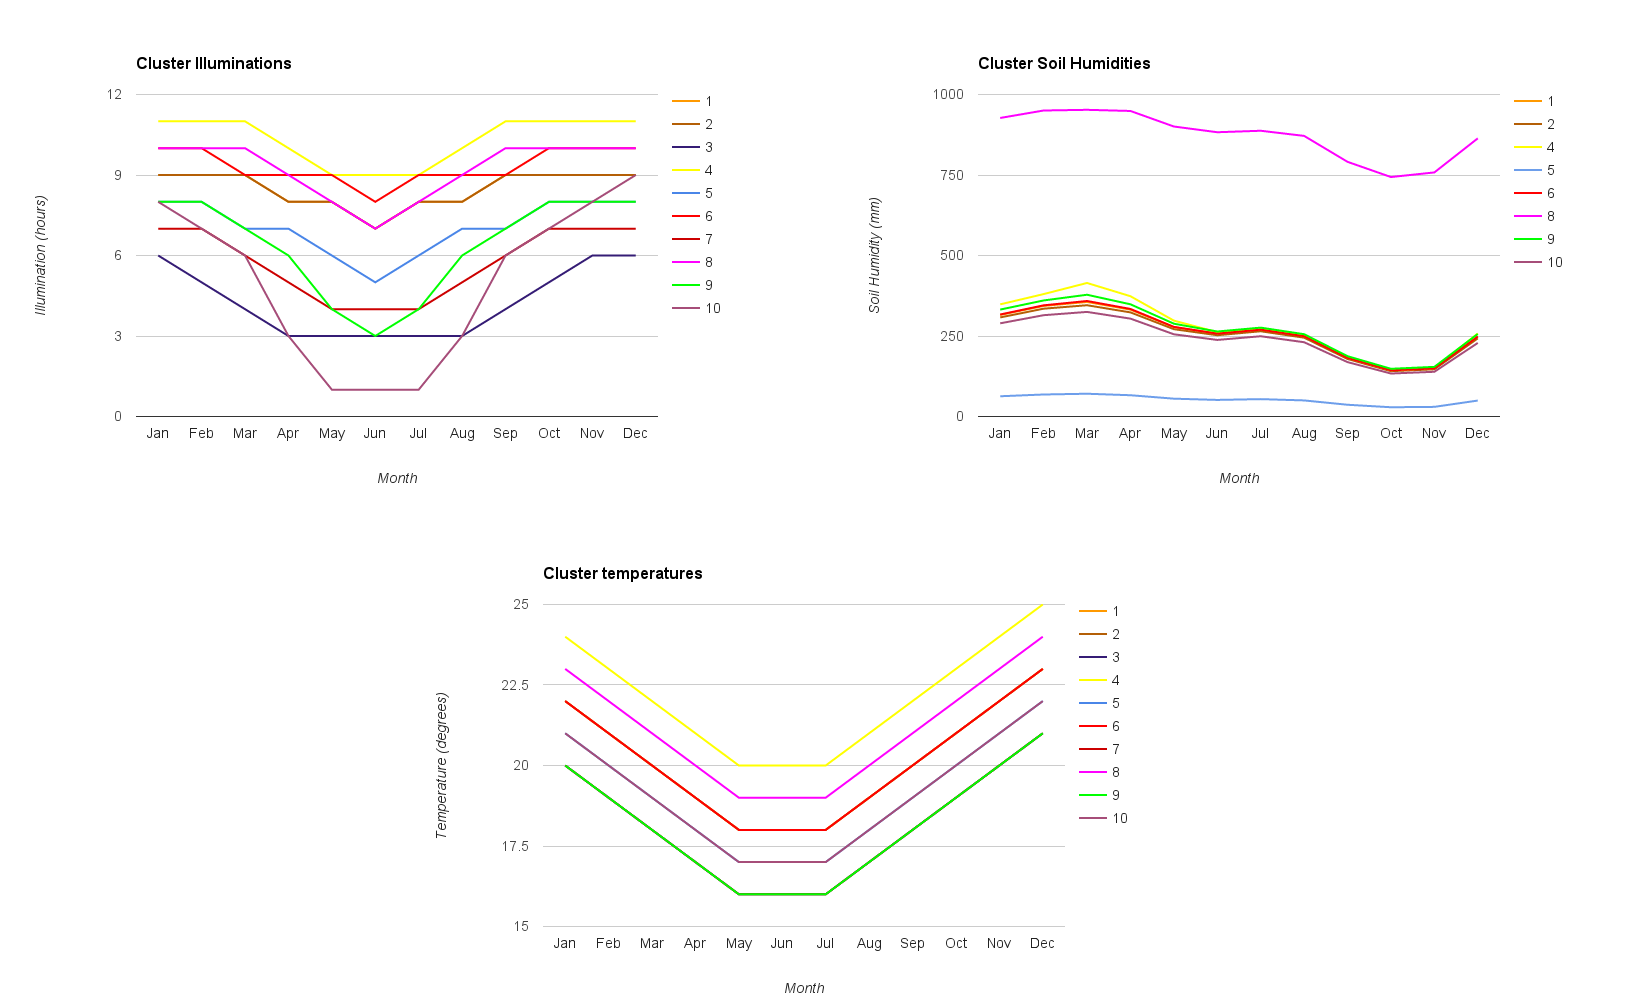
\includegraphics[width=\textwidth]{results_tropical_clusters_hum_temp_illum.png}
	\caption{ Tropical rainforest: Cluster illuminations (top-left). soil humidities (top-right) and temperatures (bottom) for each terrain cluster with color coding to match that of the cluster overlay in figure \ref{fig:results_tropical_terrain_clusters}. Note that soil humidity data is removed for clusters (3 and 7) as the corresponding values are too small.}
	\label{fig:results_tropical_cluster_hum_temp_illum}
\end{figure}

\definecolor{trop_cluster_1}{rgb}{0.8,0.4,0.0}
\definecolor{trop_cluster_2}{rgb}{0.6,0.4,0.4}
\definecolor{trop_cluster_3}{rgb}{0.0,0.2,0.4}
\definecolor{trop_cluster_4}{rgb}{1.0,1.0,0.4}
\definecolor{trop_cluster_5}{rgb}{0.0,0.6,1.0}
\definecolor{trop_cluster_6}{rgb}{1.0,0.0,0.0}
\definecolor{trop_cluster_7}{rgb}{0.8,0.2,0.0}
\definecolor{trop_cluster_8}{rgb}{1.0,0.4,0.8}
\definecolor{trop_cluster_9}{rgb}{0.0,0.8,0.4}
\definecolor{trop_cluster_10}{rgb}{0.8,0.4,1.0}

\begin{table}[h]
  \centering
	    \begin{tabular}{|p{5cm}|p{5cm}|p{5cm}|}
		\hline	
  	    \textbf{Cluster ID} & \textbf{Slope (degrees)} & \textbf{Coverage area (\% of terrain)} \\
  	    \hline	
		\cellcolor{trop_cluster_1} 1 & 22.3 & 19.3 \\
		\hline
		\cellcolor{trop_cluster_2} 2 & 32.2704 & 16.2 \\
		\hline
		\cellcolor{trop_cluster_3} 3 & 69.092 & 4.7 \\
		\hline
		\cellcolor{trop_cluster_4}4 & 2.95581 & 18.1 \\
		\hline
		\cellcolor{trop_cluster_5} 5 & 42.9369 & 4.8 \\
		\hline
		\cellcolor{trop_cluster_6} 6 & 11.8319 & 22.1 \\
		\hline
		\cellcolor{trop_cluster_7} 7 & 54.1674 & 6.0 \\
		\hline
		\cellcolor{trop_cluster_8} 8 & 8.0803 & 2.1 \\
		\hline
		\cellcolor{trop_cluster_9} 9 & 14.0102 & 2.5 \\
		\hline
		\cellcolor{trop_cluster_10} 10 & 32.1679 & 3.8 \\
		\hline
		\end{tabular}
		\caption{Tropical rainforest: Cluster slope and coverage area with color coding matching the cluster overlay in figure \ref{fig:results_tropical_terrain_clusters}.}
	  \label{tab:results_tropical_cluster_slope_covarea}
\end{table}

\subsection{Vegetation}

\subsection{Performance}


